\documentclass[aspectratio=169, 9pt]{beamer}\usepackage[]{graphicx}\usepackage[]{color}
% maxwidth is the original width if it is less than linewidth
% otherwise use linewidth (to make sure the graphics do not exceed the margin)
\makeatletter
\def\maxwidth{ %
  \ifdim\Gin@nat@width>\linewidth
    \linewidth
  \else
    \Gin@nat@width
  \fi
}
\makeatother

\definecolor{fgcolor}{rgb}{0.345, 0.345, 0.345}
\newcommand{\hlnum}[1]{\textcolor[rgb]{0.686,0.059,0.569}{#1}}%
\newcommand{\hlstr}[1]{\textcolor[rgb]{0.192,0.494,0.8}{#1}}%
\newcommand{\hlcom}[1]{\textcolor[rgb]{0.678,0.584,0.686}{\textit{#1}}}%
\newcommand{\hlopt}[1]{\textcolor[rgb]{0,0,0}{#1}}%
\newcommand{\hlstd}[1]{\textcolor[rgb]{0.345,0.345,0.345}{#1}}%
\newcommand{\hlkwa}[1]{\textcolor[rgb]{0.161,0.373,0.58}{\textbf{#1}}}%
\newcommand{\hlkwb}[1]{\textcolor[rgb]{0.69,0.353,0.396}{#1}}%
\newcommand{\hlkwc}[1]{\textcolor[rgb]{0.333,0.667,0.333}{#1}}%
\newcommand{\hlkwd}[1]{\textcolor[rgb]{0.737,0.353,0.396}{\textbf{#1}}}%
\let\hlipl\hlkwb

\usepackage{framed}
\makeatletter
\newenvironment{kframe}{%
 \def\at@end@of@kframe{}%
 \ifinner\ifhmode%
  \def\at@end@of@kframe{\end{minipage}}%
  \begin{minipage}{\columnwidth}%
 \fi\fi%
 \def\FrameCommand##1{\hskip\@totalleftmargin \hskip-\fboxsep
 \colorbox{shadecolor}{##1}\hskip-\fboxsep
     % There is no \\@totalrightmargin, so:
     \hskip-\linewidth \hskip-\@totalleftmargin \hskip\columnwidth}%
 \MakeFramed {\advance\hsize-\width
   \@totalleftmargin\z@ \linewidth\hsize
   \@setminipage}}%
 {\par\unskip\endMakeFramed%
 \at@end@of@kframe}
\makeatother

\definecolor{shadecolor}{rgb}{.97, .97, .97}
\definecolor{messagecolor}{rgb}{0, 0, 0}
\definecolor{warningcolor}{rgb}{1, 0, 1}
\definecolor{errorcolor}{rgb}{1, 0, 0}
\newenvironment{knitrout}{}{} % an empty environment to be redefined in TeX

\usepackage{alltt}

% \transdissolve[duration=0.2] % Only works with Adobe Acrobat

% \mode<handout>

% Some important packages
\usepackage{epstopdf}
\hypersetup{colorlinks=false, allcolors=purple}
\usepackage{booktabs}
\linespread{1.3}
\usepackage{tabularx}
\usepackage{makecell} % For makecell within tables
\usepackage{geometry}
\usepackage{algorithm2e}
\usepackage{amsmath, amssymb}
% Mathematical functions
% DELETED!
\renewcommand{\Pr}[1]{{\mathbb{P}\left(#1\right) }}
% DELETED!
% DELETED!
% DELETED!
% DELETED!
% DELETED!

% DELETED!
\newcommand{\sufstats}[1]{s\left(#1\right)}
\renewcommand{\exp}[1]{\mbox{exp}\left\{#1\right\}}
\newcommand{\transpose}[1]{{#1}^\mathbf{t}}

% Objects
% DELETED!
% DELETED!
\newcommand{\Graph}{\mathbf{G}}
\newcommand{\graph}{\mathbf{g}}
\newcommand{\GRAPH}{\mathcal{G}}
\newcommand{\Adjmat}{Y}
\newcommand{\adjmat}{y}
\newcommand{\ADJMAT}{\mathcal{Y}}

\newcommand{\INDEPVAR}{\mathcal{X}}
\newcommand{\Indepvar}{X}
\newcommand{\indepvar}{x}

\newcommand{\normconst}{\kappa\left(\params, \Indepvar\right)}

\graphicspath{{./figures/}{.}{./terms/}}


%% NEED THIS FOR CANCY TEX
\usepackage{pstricks}

% Colors
\definecolor{USCCardinal}{HTML}{990000} % 153 0 0 in RGB
\definecolor{USCGold}{HTML}{FFCC00}
\definecolor{USCGray}{HTML}{CCCCCC}

% To use the function \sout
\usepackage{ulem}
\usepackage{tabularx, booktabs}

% \bibliography{bibliography.bib}

\def\ergmito{ERGM\textit{ito}}
\def\ergmitos{\ergmito{}\textit{s}}
% Mathematical functions
\newcommand{\isone}[1]{{\boldsymbol{1}\left( #1 \right)}}
\renewcommand{\Pr}[1]{{\mathbb{P}\left(#1\right) }}
\newcommand{\f}[1]{{f\left(#1\right) }}
\newcommand{\Prcond}[2]{{\mathbb{P}\left(#1\vphantom{#2}\;\right|\left.\vphantom{#1}#2\right)}}
\newcommand{\fcond}[2]{{f\left(#1|#2\right) }}
\newcommand{\Expected}[1]{{\mathbb{E}\left\{#1\right\}}}
\newcommand{\ExpectedCond}[2]{{\mathbb{E}\left\{#1\vphantom{#2}\right|\left.\vphantom{#1}#2\right\}}}
\renewcommand{\exp}[1]{\mbox{exp}\left\{#1\right\}}

\newcommand{\Likelihood}[2]{\text{L}\left(#1 \left|\vphantom{#1}#2\right.\right)}

% Mathematical Annotation -------------------------------
% Modify this so that it matches the P01 convention overall

% Tree
\newcommand{\phylo}{\Lambda{}} % The actual tree
\newcommand{\aphylo}{D{}}      % The annotated phylogenetic tree
\newcommand{\aphyloObs}{\tilde \aphylo{}} % The observed annotated phylogenetic tree
\newcommand{\parent}[1]{\mathbf{p}\left(#1\right)}
\newcommand{\offspring}[1]{\mathbf{O}\left(#1\right)}
\newcommand{\nodes}{\mathcal{N}{}}
\newcommand{\edges}{\mathcal{E}{}}

\newcommand{\class}[1]{C_{#1}{}}

% Annotations
\newcommand{\Ann}{\mathbf{X}{}} % Matrix of "real" annotations
\newcommand{\ann}[1]{x_{#1}{}} % single element of "real" annotations
\newcommand{\constraints}{\mathcal{C}{}} % Taxon constraints

% Obs Annotations
\newcommand{\AnnObs}{\mathbf{Z}{}}%{Z{}} \mathbf{X}^{obs}{}
\newcommand{\annObs}[1]{z_{#1}{}}%{z{}}  x_{#1}^{obs

% Pred. Annotations
\newcommand{\AnnPred}{\hat X{}}
\newcommand{\annPred}[1]{\hat x_{#1}}

% Leaf nodes
\newcommand{\Leaf}{L{}}

% Shortest path
\newcommand{\Geodesic}{\text{T}{}}
\newcommand{\geodesic}{\tau{}}

\newcommand{\Params}{\Omega{}}
\newcommand{\params}{\omega{}}

% Parameters
\newcommand{\gain}{\mu_{01}{}}
\newcommand{\loss}{\mu_{10}{}}
\newcommand{\misszero}{\psi_{01}{}}
\newcommand{\missone}{\psi_{10}{}}
\newcommand{\proot}{\pi}


\usepackage[style=authoryear-comp]{biblatex}
\addbibresource{bibliography.bib}
% \renewcommand{\bibsection}{\subsubsection*{\bibname } }


% Styles
\usepackage{xcolor}
\usepackage{colortbl}
\definecolor{suffstat}{RGB}{10,159,0}
\definecolor{normconst}{RGB}{87,38,231}
\setbeamercolor{conclusions}{bg=usclightgray!60!white, fg=uscdarkgray}

% Noice!
\usetheme{usckeck}

\title[Computational Stats]{
{\small Seminario IMC UC}\linebreak
Predicción de funciones genéticas utilizando evidencia experimental y árboles filogenéticos: Un modelo evolutivo
\linebreak o {\small Ciencia de datos en la práctica}
}
\author[ggvy.cl]{George G Vega Yon\linebreak Candidato a Doctor}
\institute[USC-PREVMED]{University of Southern California, Department of Preventive Medicine}
\date{Abril 14, 2020}

% Some definitions
\def\cursection{\frame{\frametitle{Contents}\tableofcontents[current]}}
\newcommand{\ergmpkg}[0]{\texttt{ergm}}
\newcommand{\ergmitopkg}[0]{\texttt{ergmito}}
\newcommand{\aphylopkg}[0]{\texttt{aphylo}}
\graphicspath{{.}{fig/}}


% ------------------------------------------------------------------------------
% ------------------------------------------------------------------------------
% --------------------------- END OF PREAMBLE ----------------------------------
% ------------------------------------------------------------------------------
% ------------------------------------------------------------------------------
\setbeamertemplate{note page}[plain]
%\setbeameroption{show notes}
\usepackage{pgfpages}
% \setbeameroption{show notes on second screen}

\newcommand{\hlc}[2]{{\only<#1>{\cellcolor{gray!50} #2}}}
\newcommand{\nhlc}[2]{{\only<#1>{#2}}}
\IfFileExists{upquote.sty}{\usepackage{upquote}}{}
\begin{document}

% ------------------------------------------------------------------------------
\begin{frame}%[noframenumbering]
\maketitle
\end{frame}


% ------------------------------------------------------------------------------
\section{Introduction}

\begin{frame}
\frametitle{Acerca de}
\begin{itemize}
\item Ingeniero comercial UAI \pause$\to$ Economista Caltech \pause$\to$ Estadística Computacional USC. \pause
\item Funcionario público (5 años repartidos entre Mineduc, MDS, S Pensiones).\pause
\item Nerd de R (fundé el grupo de usuarios de R en Chile el 2013).\pause
\item Casado, 2 hijos, 1 perro.\pause
\item Varios años en proyectos de ``Data Science''.\pause
\item Mi investigación se centra en estadística computacional con énfasis en: Computación en paralelo, análisis de redes sociales, desarrollo de software, y métodos gral.
\end{itemize}\pause

Más en \textbf{http://ggvy.cl}.

\end{frame}

\begin{frame}[t]
\usebeamertemplate{section intro}{}{}
\textcolor{uscgold}{
\Large {\bf On the prediction of gene functions using phylogenetic trees} \vskip0.25em
\large \textit{Joint with}: Paul D Thomas, Paul Marjoram, Huaiyu Mi, Duncan Thomas, and John Morrison
}
\end{frame}

% ------------------------------------------------------------------------------
\begin{frame}
\frametitle{Genes}

Encode the synthesis of genetic products that ultimately are related to a
particular aspect of life, for example

\def\tmpwidth{.9\linewidth}

\begin{table}
\begin{tabular}{*{3}{m{.31\linewidth}<{\centering}}}
\onslide<2->\bf Molecular function & %
\onslide<3->\bf Cellular component & %
\onslide<4->\bf Biological process \\
\onslide<2->\href{http://amigo.geneontology.org/amigo/term/GO:0005215}{Active transport GO:0005215}& %
\onslide<3->\href{http://amigo.geneontology.org/amigo/term/GO:0004016}{Mitochondria GO:0004016} & %
\onslide<4->\href{http://amigo.geneontology.org/amigo/term/GO:0060047}{Heart contraction GO:0060047} \\
\onslide<2->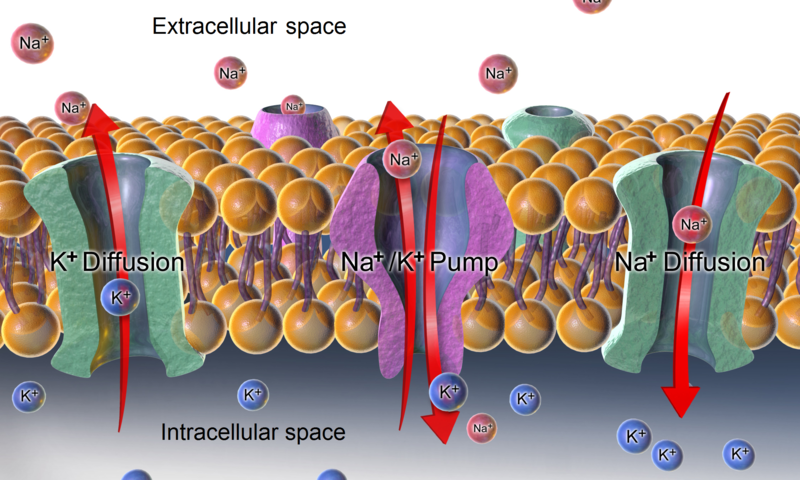
\includegraphics[width=\tmpwidth]{Sodium-potassium_pump_and_diffusion.png} & %
\onslide<3->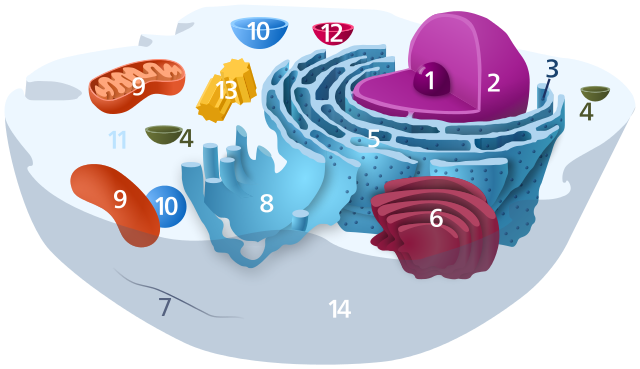
\includegraphics[width=\tmpwidth]{640px-Animal_Cell-svg.png} & % 
\onslide<4->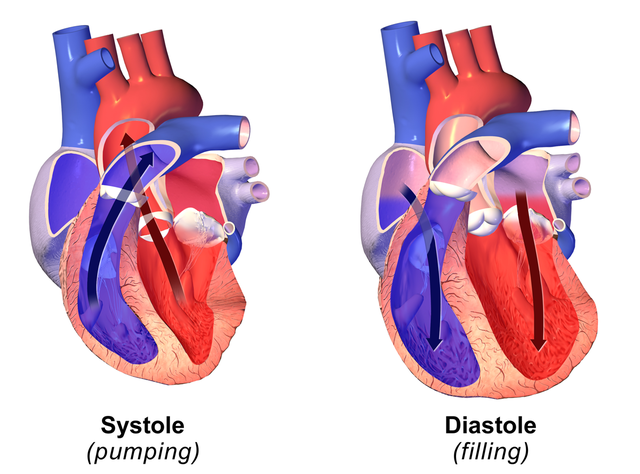
\includegraphics[width=\tmpwidth]{Systolevs_Diastole.png}
\end{tabular}
\end{table}

\end{frame}

\note[enumerate]{
\item Understanding genes means understanding biology
\item Far more than simply pursuing knowledge, this means that we can actually
use this information towards 
}


% ------------------------------------------------------------------------------
\begin{frame}[label=geneontology]
\frametitle{The Gene Ontology Project}

\begin{figure}

\includegraphics[width=.5\linewidth]{go-logo.png}
\end{figure}

\begin{itemize}[<+->]
% \item Three domains: Cellular component, molecular function, biological process.
\item The GO project has $\sim$ 44,700 validated terms  \hyperlink{aphylo-goexample}{\beamergotobutton{more}}, $\sim$ 7.3M annotations on $\sim$ 4,500 species.
\item About $\sim$ 500,000 are on human genes.
\item Roughly half of human genes ($\sim$ 10,000 / 20,000) have some
form of annotation.
\item We know something of less than 10\% of known genes (near 1.7M across species).
% \item An important effort of the GO has to do with phylogenetics...
\end{itemize}

\vfill
\hfill \textbf{source}: Statistics from \url{pantherdb.org} and \url{geneontology.org}

\end{frame}

\note[itemize]{
\item The Gene Ontology Project, which is an international scientific effort to develop
a knowledge base of biology from molecular level up to organism-level systems.
\begin{quote}
[\dots] develop an up-to-date, comprehensive, computational model of biological systems, from the molecular level to larger pathways, cellular and organism-level systems.
\item It has a large collection of genetic annotations from various types of evidence
including: experimentally, human curated information, and machine inferred.
\end{quote}

\item A long way since 1999 (20 years), there's still a lot to learn
\item This information has been crucial for bio-medical research (e.g. translating
GWAS to treatment.)
}


\begin{frame}[label=aphylo-goexample]
\frametitle{The Gene Ontology Project}

Example of GO term

\begin{table}
\footnotesize
\begin{tabular}{lm{.6\linewidth}}
\toprule
\textbf{Accession} & GO:0060047 \\
\textbf{Name} & heart contraction \\
\textbf{Ontology} & biological\_process \\
\textbf{Synonyms} & heart beating, cardiac contraction, hemolymph circulation \\
\textbf{Alternate} & IDs None \\
\textbf{Definition} & The multicellular organismal process in which the heart decreases in volume in a 
characteristic way to propel blood through the body. Source: GOC:dph \\
\bottomrule
\end{tabular}
\caption{Heart Contraction Function. source: \href{http://amigo.geneontology.org/amigo/term/GO:0060047}{amigo.geneontology.org}}
\end{table}%\pause

You know what is interesting about this function?

\end{frame}

% ------------------------------------------------------------------------------
\begin{frame}[t]

These four species have a gene with that function... \uncover<2->{and two of %
these are part of the same evolutionary tree!}

\vfill

\def\tmpwidth{.30\linewidth}
\begin{table}
\footnotesize
\begin{tabular}{*{2}{m{\tmpwidth}<\centering}}
\only<1>{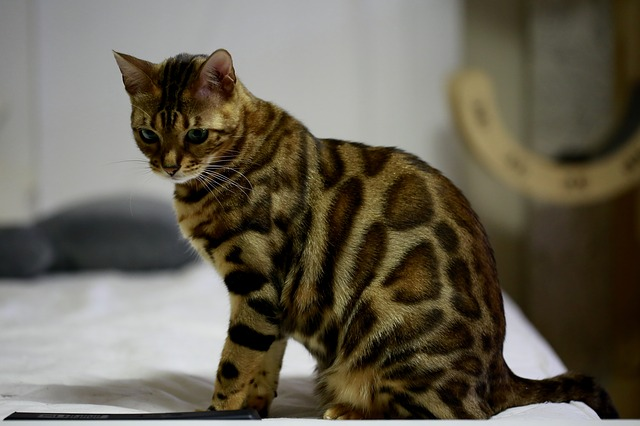
\includegraphics[width=.95\linewidth]{cat.jpg}} %
  \only<2->{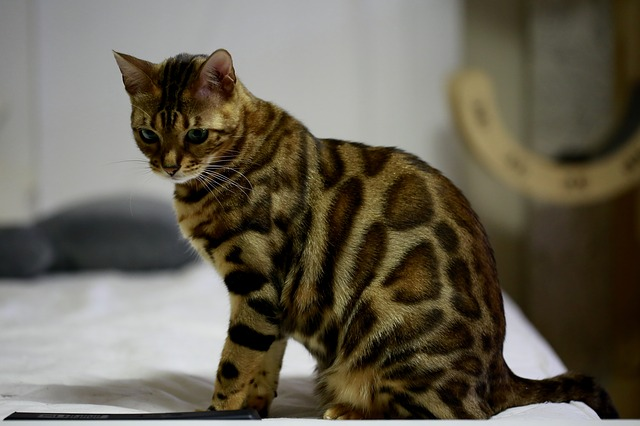
\includegraphics[width=.4\linewidth]{cat.jpg}} \linebreak Felis catus pthr10037 & %
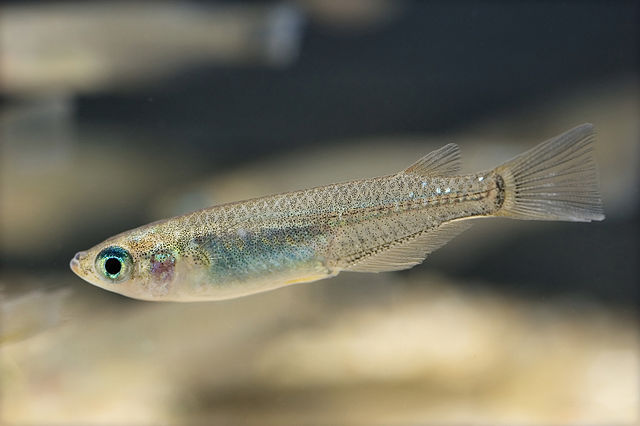
\includegraphics[width=1\linewidth]{Oryzias_latipes.jpg} \linebreak Oryzias latipes \textbf{pthr11521} \\ %
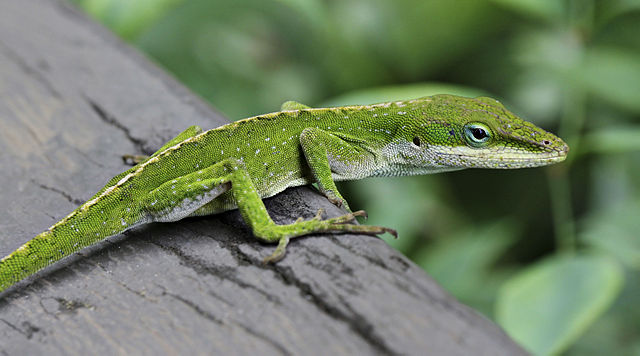
\includegraphics[width=1\linewidth]{Anole_Lizard.jpg} \linebreak Anolis carolinensis \textbf{pthr11521} & %
\only<1>{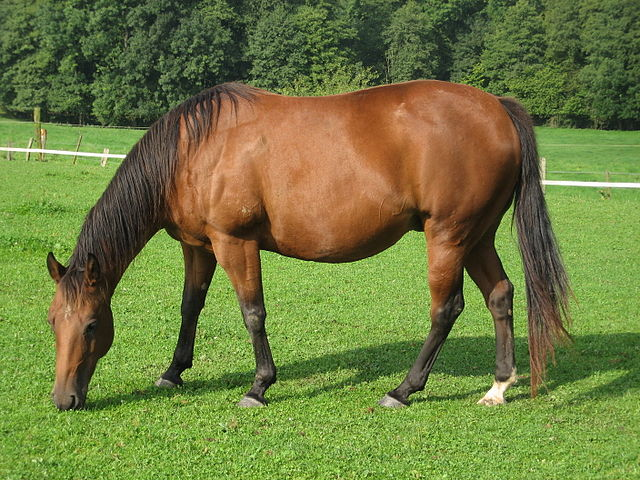
\includegraphics[width=.725\linewidth]{horse.jpg}} %
  \only<2->{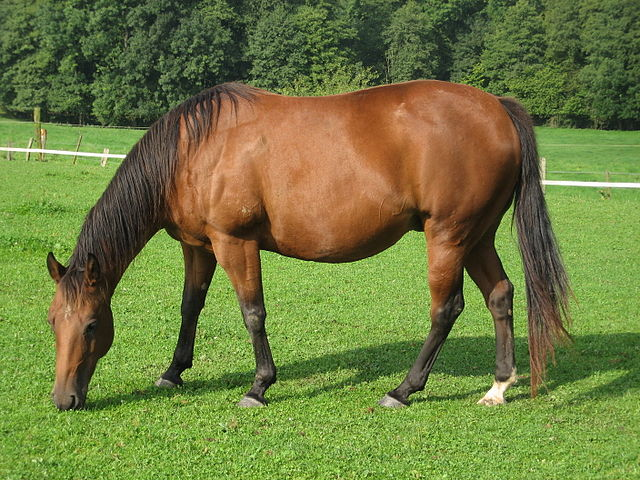
\includegraphics[width=.4\linewidth]{horse.jpg}} \linebreak Equus caballus pthr24356
\end{tabular}
\end{table}

\vfill \hfill \hyperlink{geneontology}{\beamerreturnbutton{go back}}

\end{frame}

% ------------------------------------------------------------------------------
\begin{frame}

\begin{figure}
\centering
{\footnotesize
\def\svgwidth{.7\linewidth}
\input{fig/Phylogenetic_tree-wiki.pdf_tex}
}
\caption{A phylogenetic tree of living things, based on RNA data and proposed by Carl Woese, showing the separation of bacteria, archaea, and eukaryotes (\href{https://en.wikipedia.org/wiki/File:Phylogenetic_tree.svg}{wiki})}
\end{figure}
\end{frame}

\note[enumerate]{
\item Phylogenetic trees show evolutionary relationships between species
\item Traditionally, we think about these based on say physical features, 
nowadays we build trees based on genetic distances between species.
}

% % ------------------------------------------------------------------------------
% \begin{frame}
% \begin{figure}
% \centering
% \def\svgwidth{.8\linewidth}
% \input{fig/Ortholog_paralog_analog_examples.pdf_tex}
% \end{figure}
% \end{frame}


% ------------------------------------------------------------------------------
\begin{frame}[t]
\frametitle{Phylogenetic Trees: The PANTHER classification system}
\begin{minipage}{.4\linewidth}
\pause\small
\begin{itemize}[<+->]
\item The PANTHER project (part of GO) provides information about evolutionary structure of 1.7 million
genes
\item These genes are grouped in 15,524 phylogenetic trees (families)
\item A single family can host multiple species
\end{itemize}
\end{minipage}
\hfill
\begin{minipage}{.5\linewidth}
\uncover<5->{
\begin{knitrout}
\definecolor{shadecolor}{rgb}{0.969, 0.969, 0.969}\color{fgcolor}\begin{figure}

{\centering 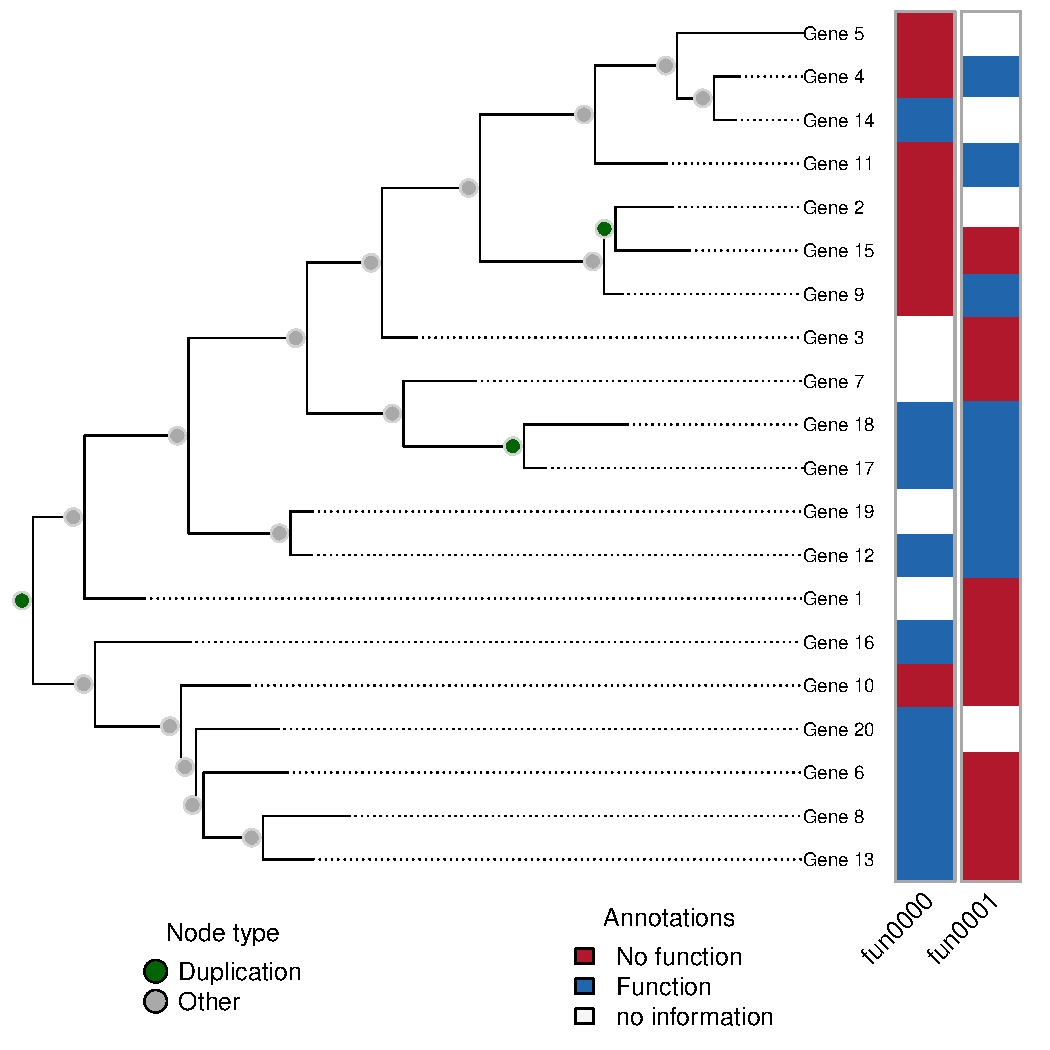
\includegraphics[width=.85\linewidth]{figure/random-tree-1} 

}

\caption[Simulated phylogenetic tree and gene annotations]{Simulated phylogenetic tree and gene annotations.}\label{fig:random-tree}
\end{figure}


\end{knitrout}
}
\end{minipage}
\end{frame}

\note[enumerate]{
\item Here we have an example of a (simulated) phylogenetic tree.
\item We will see this a couple of times during the presentation
\item This figure summarizes the information that I will be using
to infer gene functions:
\begin{itemize}
\item The tip nodes (leafs) are modern (known) genes
\item In general, The color bars next to each gene represent genetic annotations
(GO terms) in three different states: Has the function (blue), does not have the
function (red), and no information (white)
\item Each interior node represent ancestors which are classify as 
duplication/speciation/or horizontal transfer nodes
\item This is an hypothesis regarding to what type of event lead
to a split in the family.
\item we mostly care about whether these are duplication nodes not
since we believe that functional gain and loses are more likely
to happen at this stage.
\end{itemize}
}


% ------------------------------------------------------------------------------
\begin{frame}[label = duplicationvsspeciation]
\frametitle{Speciation}
\begin{figure}
\centering
\def\svgwidth{.8\linewidth}
\tiny
% Source 
\input{fig/Drosophila_speciation_experiment.pdf_tex}
\caption{\cite{Dodd1989}: After one year of isolation, flies showed a significant level or assortativity in mating (\href{https://commons.wikimedia.org/wiki/File:Drosophila_speciation_experiment.svg}{wikimedia})}
\end{figure}

\vfill\hfill \hyperlink{aphylographicalview}{\beamerreturnbutton{go back}}

\end{frame}

\begin{frame}
\frametitle{Duplication}
\begin{figure}
\centering
\def\svgwidth{.6\linewidth}
\tiny
% Source : https://en.wikipedia.org/wiki/File:Evolution_fate_duplicate_genes_-_vector.svg
\input{fig/Evolution_fate_duplicate_genes_-_vector.pdf_tex}
\caption{A key part of molecular innovation, gene duplication provides opportunity for new functions to emerge (\href{https://en.wikipedia.org/wiki/File:Evolution_fate_duplicate_genes_-_vector.svg}{wikimedia})}
\end{figure}

\vfill\hfill \hyperlink{aphylographicalview}{\beamerreturnbutton{go back}}

\end{frame}

% %
% \frame{
% \centering
% \Large
% We can use \vspace{.5cm}
% 
% \textcolor{usccardinal}{ {\Huge evolutionary trees}} \vspace{.5cm}
% 
% to inform a model for predicting \vspace{.5cm}
% 
%  \textcolor{usccardinal}{{ \Huge genetic annotations!}}
% }



\note[enumerate]{

There various approaches for this, some to highlight
\begin{itemize}%[<+->]
\item Text analysis like in \cite{Pesaranghader2016}
\item Protein-protein interaction networks like in \cite{Oliver2000,Piovesan2015}.
\item Phylogenetic based like SIFTER \cite{Engelhardt2005,Engelhardt2011}.
\begin{itemize}
\item Parameters to estimate: $2^{2P}$, where $P$ is the number of functions.
\end{itemize}
\end{itemize}

\vfill \hfill (a nice literature review in \cite{Jiang2016,Yu2018})

\item The last one being the most closely related to what we propose here
(details to be shown).
\item , functions are modeled using a transition matrix in
a Markov continuous model.
\item The main problem with this is that the computational complexity
of the model grows horribly (estimating a model with a 100 functions)
takes literally infinite time.
\item B/c of this, they truncate some of their modelling and work with
small sets of up to 5 functions in a single tree (for example).
\item One key point of most of these models is that these provide a
point estimate rather than a distribution, and mostly a binary
estimate of the annotation (yes/no).
}

% ------------------------------------------------------------------------------
\begin{frame}[label=aphylographicalview]
\frametitle{An evolutionary model of gene functions}

\definecolor{rootnode}{RGB}{0,159,211}
\definecolor{innernode}{RGB}{90,159,89}
\definecolor{leafnode}{RGB}{255,107,0}

\begin{minipage}{.48\linewidth}
\begin{itemize}
	\item<2-> \textcolor{rootnode}{Initial (spontaneous) gain of function}.
	\item<3-> \textcolor{innernode}{Loss/gain of offspring depends on: (a) the state of their parents ({\bf (discrete) Markov process}), and (b) the type of node}
	\item<4-> \textcolor{leafnode}{We control for human error.}
\end{itemize}
\end{minipage}
%
\begin{minipage}{.50\linewidth}
\begin{figure}
	\footnotesize
	\centering
	\def\svgwidth{.9\linewidth}
	\input{fig/aphylo.pdf_tex}
\end{figure}
\end{minipage}

\vspace{1.5cm}

% \uncover<5->{We implemented the model using Felsenstein's' pruning algorithm (linear complexity) in the
% R package \aphylopkg{}.} % \hyperlink{aphylopkg}{\beamergotobutton{more}}.}

\vfill\hfill \hyperlink{other-models}{\beamergotobutton{other models}}
\hyperlink{aphyloalgorithmicview}{\beamergotobutton{other view}}

\end{frame}

\note[enumerate]{
\item In the version of the qual document you saw an implementation of the model
that did not incorporated information regarding the node types, but that is trivially
added by just adding a separate gain/loss parameter per type
\item Another venue we have explored is accounting for publication bias, most
annotations are of the positive type (has function), but few are (no function).
\item we have failed in the last tests.
\item The model has been thoroughly tested. In particular, we did a large scale
simulation study in which we used all 15,000 trees from panther to simulate
annotations and then fitted our model using MCMC to check for bias and coverage
probabilities (which are available in the paper)
\item The experiment was carried out using USC's High Performance Computing
cluster with the R package slurmR (described in the document).
\item Now, I will show you more recent information in which we take 
data from PantherDB with GO annotations and fit a large pooled model.
}

% ------------------------------------------------------------------------------
\begin{frame}[label=math]
\frametitle{Formally}

\small

We need to calculate the probability of observing $\aphyloObs = (\phylo, \AnnObs)$ (a partially annotated phylogeny) as a function of the model parameters $\psi$ (mislabel), $\mu$ (gain/loss), $\pi$ (root node):

\begin{itemize}
\item Probability of the induced sub-tree:

\begin{equation} 
\label{eq:interior1}
{\color{blue}\Prcond{\aphyloObs_n}{\ann{n}, \psi, \mu}} =  \quad\prod_{m \in \offspring{n}} \Prcond{\aphyloObs_{m}}{\ann{n}},
\end{equation}
where
\begin{equation*}
\Prcond{\aphyloObs_{m}}{\ann{n}} = \left\{\begin{array}{ll}
	\sum_{\ann{m}\in\{0,1\}}{\color{blue}\Prcond{\aphyloObs_m}{\ann{m}, \psi, \mu}}\Prcond{\ann{m}}{\ann{n}, \mu} & \mbox{if $m$ is an interior node,} \\
	\sum_{\ann{m}\in\{0,1\}}\Prcond{\ann{m}}{\annObs{m}, \psi}
	\Prcond{\ann{m}}{\ann{n}, \mu} & \mbox{if $m$ is a leaf node.}
	\end{array}
	\right.
\end{equation*}

\item The exact likelihood:
\begin{equation}
\label{eq:ll}
\Likelihood{\psi, \mu, \pi}{\aphyloObs} =
\sum_{\ann{0} \in \{0,1\}} \Prcond{\ann{0}}{\pi} {\color{blue}\Prcond{\aphyloObs_0}{\ann{0},\psi,\mu}}
\end{equation}

\end{itemize}

This likelihood can be computed in $O(n)$, $n$ number of nodes. This is known as Post-order tree-traversal, or Felsenstein's Pruning algorithm.

\normalsize
\end{frame}


% ------------------------------------------------------------------------------
% \begin{frame}
% \frametitle{Skills}
% \begin{itemize}
% \item Desarrollar un paquete de R
% \item Programar algorithmo de Felsenstein en C++
% \item Estudio de simulación: Cluster de USC (400 trabajos en paralelo)
% \item Procesamiento de datos: data.table (paquete R) + expresiones regulares
% \item Visualización de datos: ape (paquete R) + dibujar a mano
% \end{itemize}
% \end{frame}
\section{Analysis}

\begin{frame}
\usebeamertemplate{section intro}{}{}
\textcolor{uscgold}{
\Large {\bf Implementation} \vskip0.25em
\large Software, algorithms, and analysis
}
\end{frame}

\begin{frame}[label=aphylopkg]
\frametitle{Implementation}

{\large Software and algorithms}
\begin{itemize}[<+->]
\item The likelihood function is computed using the C++ template library \texttt{pruner} (by-product).
\item To fit the model we use:
\begin{itemize}
\item \textit{Maximum Likelihood Estimation (MLE) and Maximum A Posteriory (MAP)}: Maximized using L-BFGS-B.
\item \textit{Markov Chain Monte Carlo (MCMC)}: Using the \texttt{fmcmc} R package (by-product), and in particular, Haario's Adaptive Metropolis.
\end{itemize}
\end{itemize}

\pause
{\large Analysis}
\begin{itemize}[<+->]
\item Conducted a large simulation study fitting 15,000 models with MCMC
\item The analysis was performed in USC's HPCC and took about 4 hours (using 400 cores, i.e. 2 month equiv to core hours)
\item We used the \texttt{slurmR} package (also by-product) to implement the pipe-line.
\end{itemize}

%\vfill\hfill \hyperlink{aphylographicalview}{\beamerreturnbutton{go back}}
\end{frame}

% % ------------------------------------------------------------------------------
% \section{Data}
% 
% \begin{frame}
% \usebeamertemplate{section intro}{}{}
% \textcolor{uscgold}{
% \Large {\bf The data} \vskip0.25em
% % \large \textit{Joint with}: Paul D Thomas, Paul Marjoram, Huaiyu Mi, Duncan Thomas, and John Morrison
% }
% \begin{frame}[t]
% \frametitle{Data}
% \begin{enumerate}
% \item A collection of $\sim$ 15,000 annotated phylogenetic trees.
% \item Including 
% \end{enumerate}
% \end{frame}

% ------------------------------------------------------------------------------
\section{Data}

\begin{frame}
\usebeamertemplate{section intro}{}{}
\textcolor{uscgold}{
\Large {\bf Data} \vskip0.25em
\large Phylogenetic trees and Experimental Annotations
}
\end{frame}

\begin{frame}
\frametitle{Data: Phylogenetic trees}



Sample of annotations (first 10 in a single tree)

\small

\begin{table}[ht]
\centering
\begin{tabular}{rrlll}
  \toprule
 & branch\_length & type & ancestor & duplication \\ 
  \midrule
AN0 &  & S & LUCA & FALSE \\ 
  AN1 & 0.06 & S & Archaea-Eukaryota & FALSE \\ 
  AN2 & 0.24 & S & Eukaryota & FALSE \\ 
  AN3 & 0.44 & S & Unikonts & FALSE \\ 
  AN4 & 0.42 & S & Opisthokonts & FALSE \\ 
  AN6 & 0.68 & D &  & TRUE \\ 
  AN9 & 0.79 & S & Amoebozoa & FALSE \\ 
  AN10 & 0.18 & D &  & TRUE \\ 
  AN15 & 0.57 & S & Dictyostelium & FALSE \\ 
  AN18 & 0.52 & S & Alveolata-Stramenopiles & FALSE \\ 
   \bottomrule
\end{tabular}
\end{table}

\end{frame}

\begin{frame}
\frametitle{Data: Node type (events)}
\begin{figure}
\centering
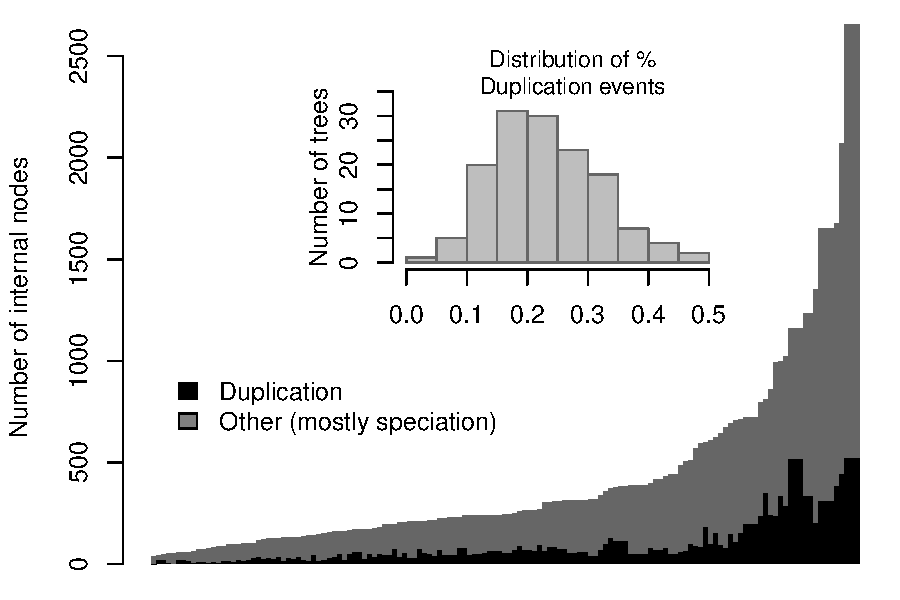
\includegraphics[width=.7\linewidth]{distribution-event-type.pdf}
\end{figure}
\end{frame}

\begin{frame}
\frametitle{Data: Annotations (example)}

This is the first 10 of $\sim$ 400,000 experimental annotations used:

\footnotesize
\begin{table}[ht]
\centering
\begin{tabular}{rllll}
  \toprule
 & Family & Id & GO term & Qualifier \\ 
  \midrule
1 & PTHR12345 & HUMAN$|$HGNC=15756$|$UniProtKB=Q9H190 & GO:0005546 &  \\ 
  2 & PTHR11361 & HUMAN$|$HGNC=7325$|$UniProtKB=P43246 & GO:0016887 & CONTRIBUTES\_TO \\ 
  3 & PTHR10782 & MOUSE$|$MGI=MGI=3040693$|$UniProtKB=Q6P1E1 & GO:0045582 &  \\ 
  4 & PTHR23086 & ARATH$|$TAIR=AT3G09920$|$UniProtKB=Q8L850 & GO:0006520 &  \\ 
  5 & PTHR32061 & RAT$|$RGD=619819$|$UniProtKB=Q9EPI6 & GO:0043197 &  \\ 
  6 & PTHR46870 & ARATH$|$TAIR=AT3G46870$|$UniProtKB=Q9STF9 & GO:1990825 &  \\ 
  7 & PTHR15204 & MOUSE$|$MGI=MGI=1919439$|$UniProtKB=Q9Z1R2 & GO:0045861 &  \\ 
  8 & PTHR22928 & DROME$|$FlyBase=FBgn0050085$|$UniProtKB=Q9XZ34 & GO:0030174 &  \\ 
  9 & PTHR35972 & HUMAN$|$HGNC=34401$|$UniProtKB=A2RU48 & GO:0005515 &  \\ 
  10 & PTHR10133 & DROME$|$FlyBase=FBgn0002905$|$UniProtKB=O18475 & GO:0097681 &  \\ 
   \bottomrule
\end{tabular}
\end{table}
\end{frame}

\begin{frame}
\frametitle{Data: Experimental Annotations}
\begin{figure}
\centering
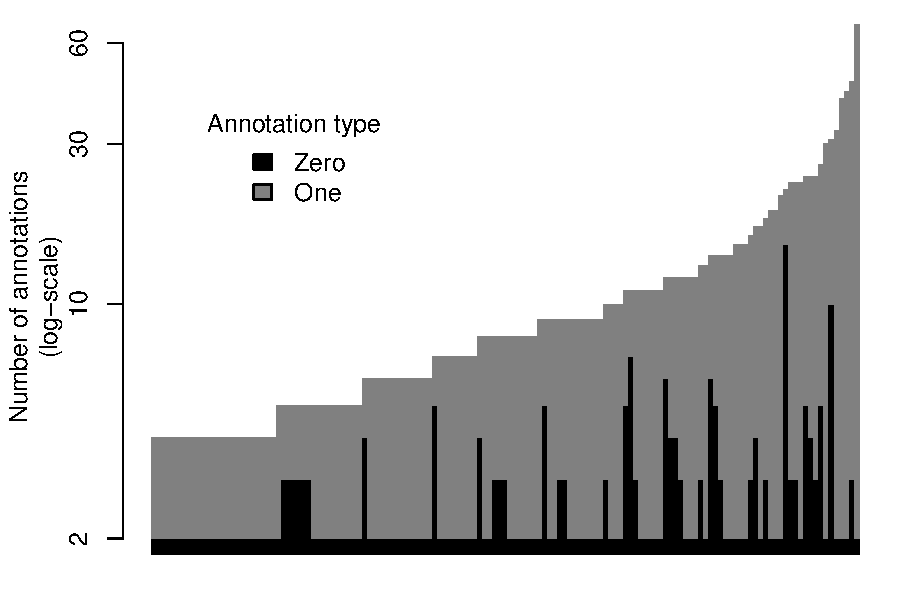
\includegraphics[width=.7\linewidth]{distribution-annotation-type.pdf}
\end{figure}
\end{frame}



% ------------------------------------------------------------------------------
\section{Results}


% ------------------------------------------------------------------------------
\begin{frame}
\usebeamertemplate{section intro}{}{}
\textcolor{uscgold}{
\Large {\bf Some preliminary results} \vskip0.25em
\large \textit{Joint with}: Paul D Thomas, Paul Marjoram, Huaiyu Mi, Duncan Thomas, and John Morrison
}
\end{frame}

\begin{frame}[t]
\frametitle{Prediction with real data}

\begin{minipage}{.39\linewidth}
\begin{table}[ht]
\centering
\scalebox{0.7}{
\begin{tabular}{ll*{2}{m{0.3\linewidth}<\centering}}
  \toprule
 & & \multicolumn{2}{c}{Prior} \\
 & & Uniform & Beta  \\ 
  \midrule
  \multicolumn{2}{l}{Mislab. prob.} \\
  & $\psi_0$ & 0.23 & 0.25 \\ 
  & $\psi_1$ & 0.01 & 0.01 \\ 
  \multicolumn{2}{l}{\textcolor<4->{usccardinal}{\textbf<4->{Gain/Loss at dupl.}}} \\
  & $\mu_{d0}$ & 0.97 & 0.96 \\ 
  & $\mu_{d1}$ & 0.52 & 0.58 \\ 
  \multicolumn{2}{l}{\textcolor<4->{usccardinal}{\textbf<4->{Gain/Loss at spec.}}} \\
  & $\mu_{s0}$ & 0.05 & 0.06 \\ 
  & $\mu_{s1}$ & 0.01 & 0.02 \\ 
  \multicolumn{2}{l}{Root node} \\
  & $\pi$ & 0.81 & 0.45  \\ 
\midrule 
\multicolumn{2}{l}{Leave-one-out AUC} \\
  & Mean & 0.69 & 0.67 \\
  & Median & 0.81 & 0.75 \\
   \bottomrule
\end{tabular}
}
\caption{Parameter estimates using different priors.} 
\end{table}
%
\end{minipage}
\begin{minipage}{.59\linewidth}
\begin{itemize}[<+->]
\item 141 pooled functions (trees) with 7,388 genes with 0/1 annotations.
\item Parameter estimates are actually probabilities.
\item Data driven results (uninformative prior).
\item \textcolor{usccardinal}{Biologically meaningful results.}
\item Took about 5 minutes each.
\end{itemize}
\end{minipage}

\end{frame}

\note[enumerate]{
\item The data used here corresponds to a subset of the trees.
\item Right now, the main criteria was: (1) must have at least one annotation
of each type, and (2) must not have large sets of siblings (this due to
numerical underflow issues, WIP)
}

% ------------------------------------------------------------------------------
\begin{frame}
\frametitle{Pooled estimation (worth it?)}

\begin{figure}
\centering
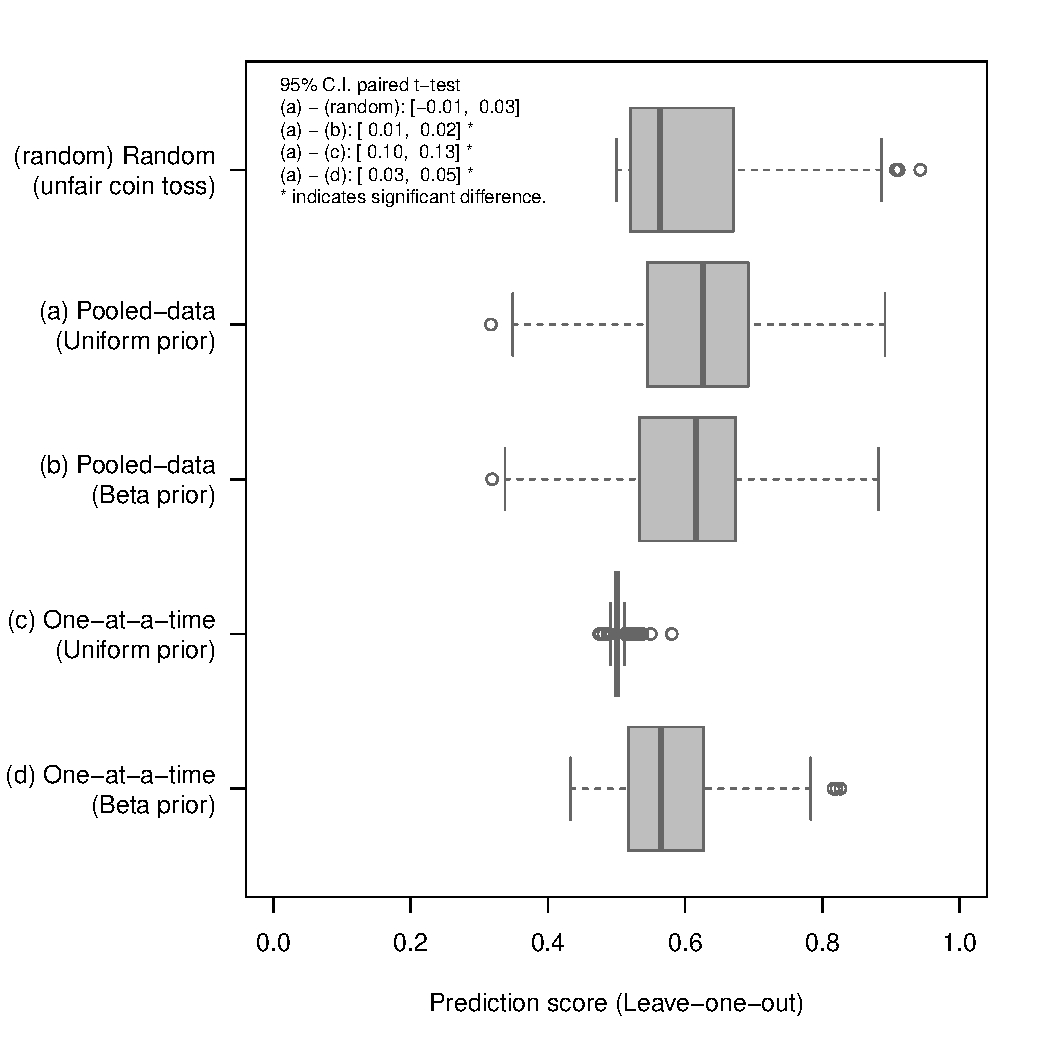
\includegraphics[width=.5\linewidth]{pooled-or-single.pdf}
\end{figure}

\end{frame}

% ------------------------------------------------------------------------------
\begin{frame}
\frametitle{Prediction with real data}

\begin{figure}
\centering
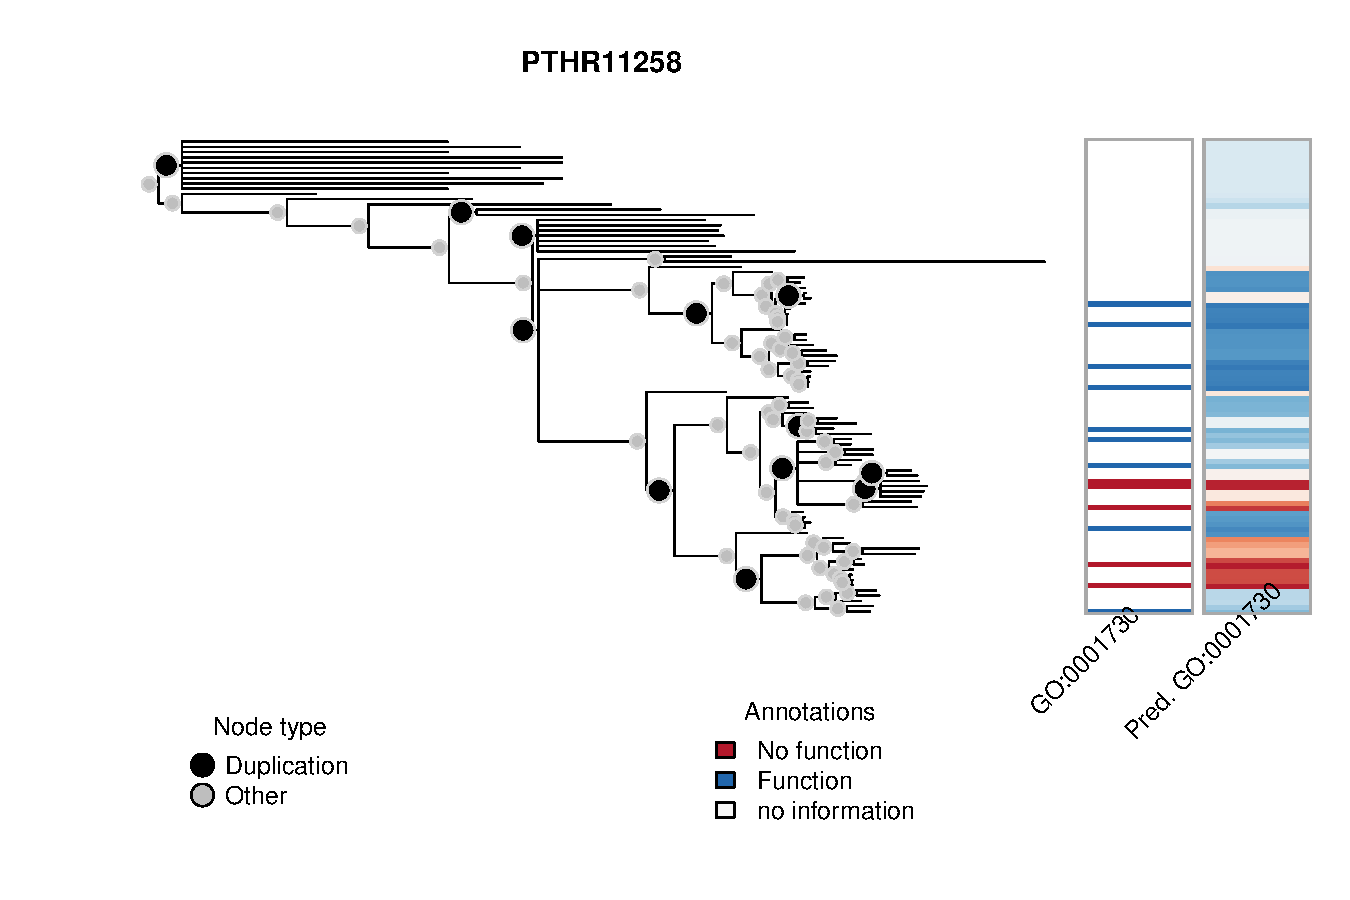
\includegraphics[width=.7\linewidth, trim = 0 1.25cm 0 .5cm, clip]{fig/example-trees-good1.pdf}
\caption{This family contains the human gene OAS1 (chromosome 12) ``a member of the 2-5A synthetase family, essential proteins involved in the innate immune response to viral infection'' (wiki)}
\end{figure}

\end{frame}

\begin{frame}
\frametitle{Prediction with real data (leave-one-out CI)}

\begin{figure}
\centering
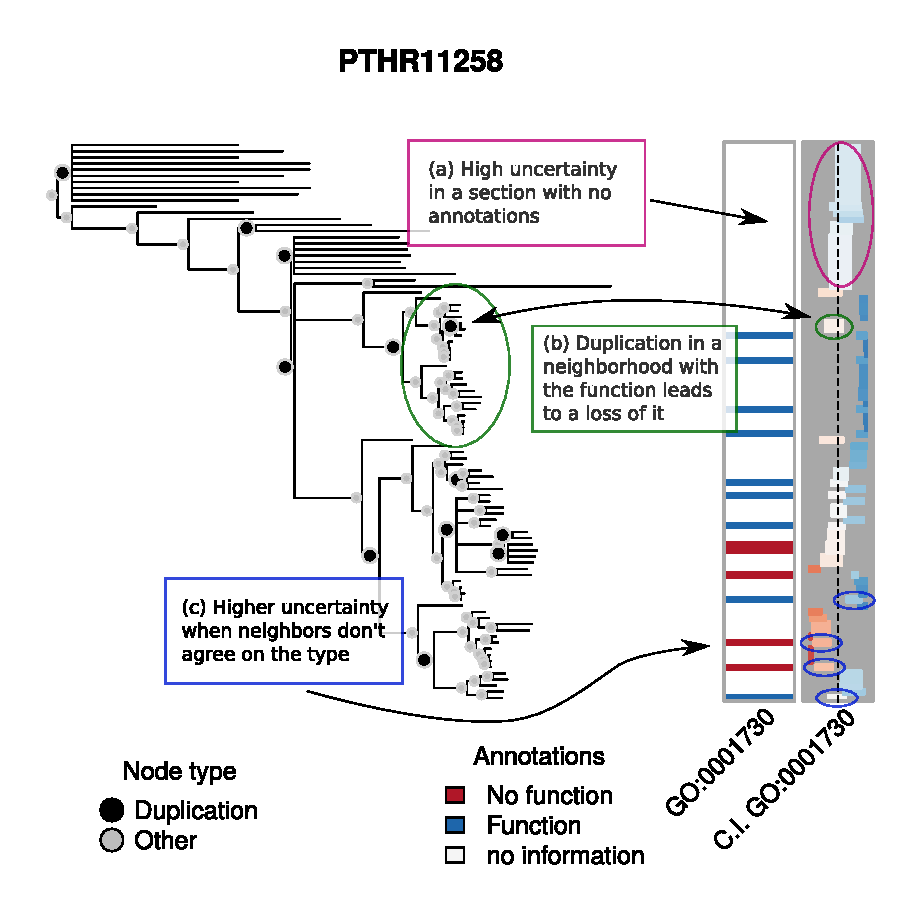
\includegraphics[width=.5\linewidth, trim = 0 .5cm 0 .5cm, clip]{example-trees-good1-loo-annotated}
% \caption{This family contains the human gene OAS1 (chromosome 12) ``a member of the 2-5A synthetase family, essential proteins involved in the innate immune response to viral infection'' (wiki)}
\end{figure}

\end{frame}
% ------------------------------------------------------------------------------
\begin{frame}[c]
\frametitle{On the prediction of gene functions using phylogenetic trees}

{\bf \large Key takeaways}
\begin{beamercolorbox}[dp=1ex]{conclusions}
\begin{itemize}
\item A parsimonious model for predicting gene functions using phylogenetics.
\item Computationally scalable. SIFTER (our benchmark)
would take about 66 years (yes, years) to estimate a model for 100 families
of size 300, we take about 5 minutes.
\item Meaningful biological results.
\item Preliminary accuracy results comparable to state-of-the-art phylo-based models.
\end{itemize}
\end{beamercolorbox}\pause


\end{frame}



% ------------------------------------------------------------------------------
\begin{frame}
\frametitle{Future Research: phylogenetic models}

\begin{itemize}
\item Make the model hierarchical when pooling trees\pause
\begin{itemize}
\item Different mutation rates per class of tree/function
\item Can be complicated to fit/justify (how many classes?)
\end{itemize}\pause
\item Use a framework similar to Exponential Random Graph Models:\pause

$$
\Prcond{\Ann=\{\ann{n1}, \ann{n2},\dots\}}{\ann{\parent{n1, \dots}}} = \frac{\exp{\mu^{T} s(\mathbf{x}|\ann{\parent{\cdot}})}}{\sum_{\mathbf{x}'}\exp{\mu^{T} s(\mathbf{x}'|\ann{\parent{\cdot}})}}
$$

\begin{itemize}
\item A generalization of the model.
\item Extends to account for joint dist of functions+siblings.
\item Can incorporate additional information such as branch lengths.
\item Yet computationally more compact compared to SIFTER (finite number of parameters).
\end{itemize}
\end{itemize}


\end{frame}

% ------------------------------------------------------------------------------
\begin{frame}[t]
\frametitle{Future Research: phylogenetic models}

Imagine that we have 3 functions (rows) and that each node has 2 siblings (columns)

\mode<beamer>{
  \begin{table}
  \begin{tabular}{llcc}
  \toprule
  & & \multicolumn{2}{c}{\bf Transitions to} \\
   & & Case 1 & Case 2 \\ \cmidrule(r){3-4}
  \multicolumn{2}{r}{\textbf{Parent} $\begin{array}{c}\mbox{A} \\ \mbox{B} \\ \mbox{C}\end{array}\left[\begin{array}{c}0 \\ 1 \\ 1\end{array}\right]$} & 
  $\left[\begin{array}{cc} %
    0 & \nhlc{1-2}{1}\hlc{3-5}{1}\nhlc{6-}{1} \\ %
    1 & \nhlc{1-3}{0}\hlc{4-5}{0}\nhlc{6-}{0} \\ %
    1 & \nhlc{1-3}{0}\hlc{4}{1}\nhlc{5-}{1} %
    \end{array}\right]$ & 
  $\left[\begin{array}{cc} %
    0 & \nhlc{-2}{1}\nhlc{4}{1}\hlc{3}{1}\hlc{5}{1}\nhlc{6-}{1} \\ %
    \nhlc{-5}{1}\hlc{6}{1}\nhlc{7-}{1} & \nhlc{-4}{0}\hlc{5}{0}\nhlc{6-}{0}\\ %
    \nhlc{-4}{0}\hlc{5}{0}\nhlc{6-}{0} & \nhlc{1-5}{1}\hlc{6}{1}\nhlc{7-}{1}%
    \end{array}\right]$ \pause \\ \midrule 
  \multicolumn{3}{l}{\textbf{Sufficient statistics}} \pause \\ 
  & \# Gains (Neofunctionalization) & 1 & 1 \pause \\
  & Only one offspring changes (yes/no) & 1 & 0 \pause \\
  & \# Changes (gain+loss) & 2 & 3 \pause \\
  & Subfunctionalization (yes/no) & 0 & 1 \\ \bottomrule
  \end{tabular}
  \end{table}
}
\mode<handout>{
  \begin{table}
  \begin{tabular}{llcc}
  \toprule
	& & \multicolumn{2}{c}{\bf Transitions to} \\
	& & Case 1 & Case 2 \\ \cmidrule(r){3-4}
	\multicolumn{2}{r}{\textbf{Parent} $\begin{array}{c}\mbox{A} \\ \mbox{B} \\ \mbox{C}\end{array}\left[\begin{array}{c}0 \\ 1 \\ 1\end{array}\right]$} & 
	$\left[\begin{array}{cc} %
	0 & 1 \\ %
	1 & 0 \\ %
	1 & 1 %
	\end{array}\right]$ & 
	$\left[\begin{array}{cc} %
	0 & 1 \\ %
	1 & 0\\ %
	0 & 1%
	\end{array}\right]$ \\ \midrule 
	\multicolumn{3}{l}{\textbf{Sufficient statistics}} \\ 
	& \# Neofunctionalizations & 1 & 1  \\
	& Only one offspring changes (yes/no) & 1 & 0 \\
	& \# Changes (gain+loss) & 2 & 3 \\
	& Subfunctionalizations (yes/no) & 0 & 1 \\ \bottomrule
  \end{tabular}
  \end{table}
}

\pause
In SIFTER, for modelling 3 functions (with offsprings conditionally independent), we need $2^{2\times 3} = 64$ parameters.

\end{frame}





% % ------------------------------------------------------------------------------
\begin{frame}
\maketitle
\begin{center}
\scalebox{2}{\textcolor{uscgold}{Thanks!}}
\end{center}
\end{frame}

\section{Data Science}

% \begin{frame}
% \frametitle{En la practica}
% Habilidades duras:
% \begin{itemize}
% \item Un lenguaje de programación.
% \item Expresiones regulares (Regex).
% \item Línea de comandos.
% \item Sistema de control de versión.
% \item Visualizar datos.
% \end{itemize}
% Habilidades blandas:
% \begin{itemize}
% \item Iterpretación de los resultados (clave).
% \item Trabajo en equipo (participar, mostrar que piensas en problemas/soluciones)
% \item Iniciativa y buena "Work ethics".
% \end{itemize}
% \end{frame}

\frame{
\frametitle{Saber interpretar los modelos}
\begin{figure}
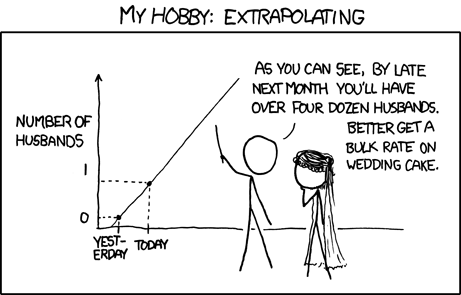
\includegraphics[width=.6\linewidth]{extrapolating.png}
\caption{Fuente: https://xkcd.com/605/}
\end{figure}
}


\frame{
\frametitle{Expresiones regulares}
\begin{figure}
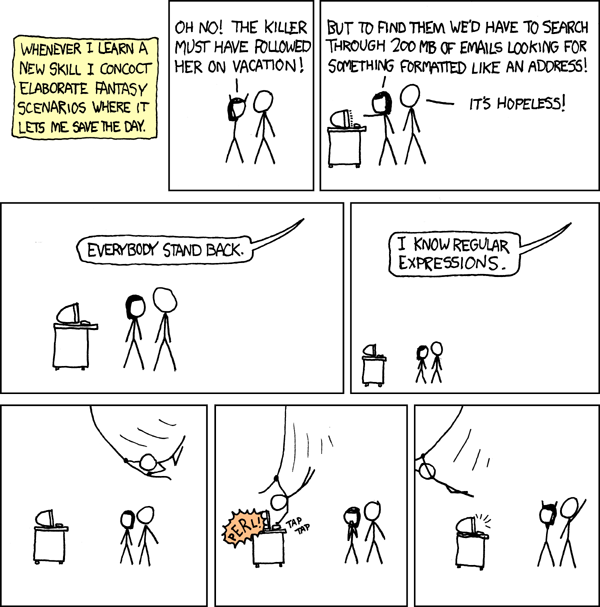
\includegraphics[width=.45\linewidth]{regular_expressions.png}
\caption{Fuente: https://xkcd.com/208/}
\end{figure}
}

\frame{
\frametitle{Data Science... Otro ``Buzzword''}
Pero si insisten...
\begin{figure}
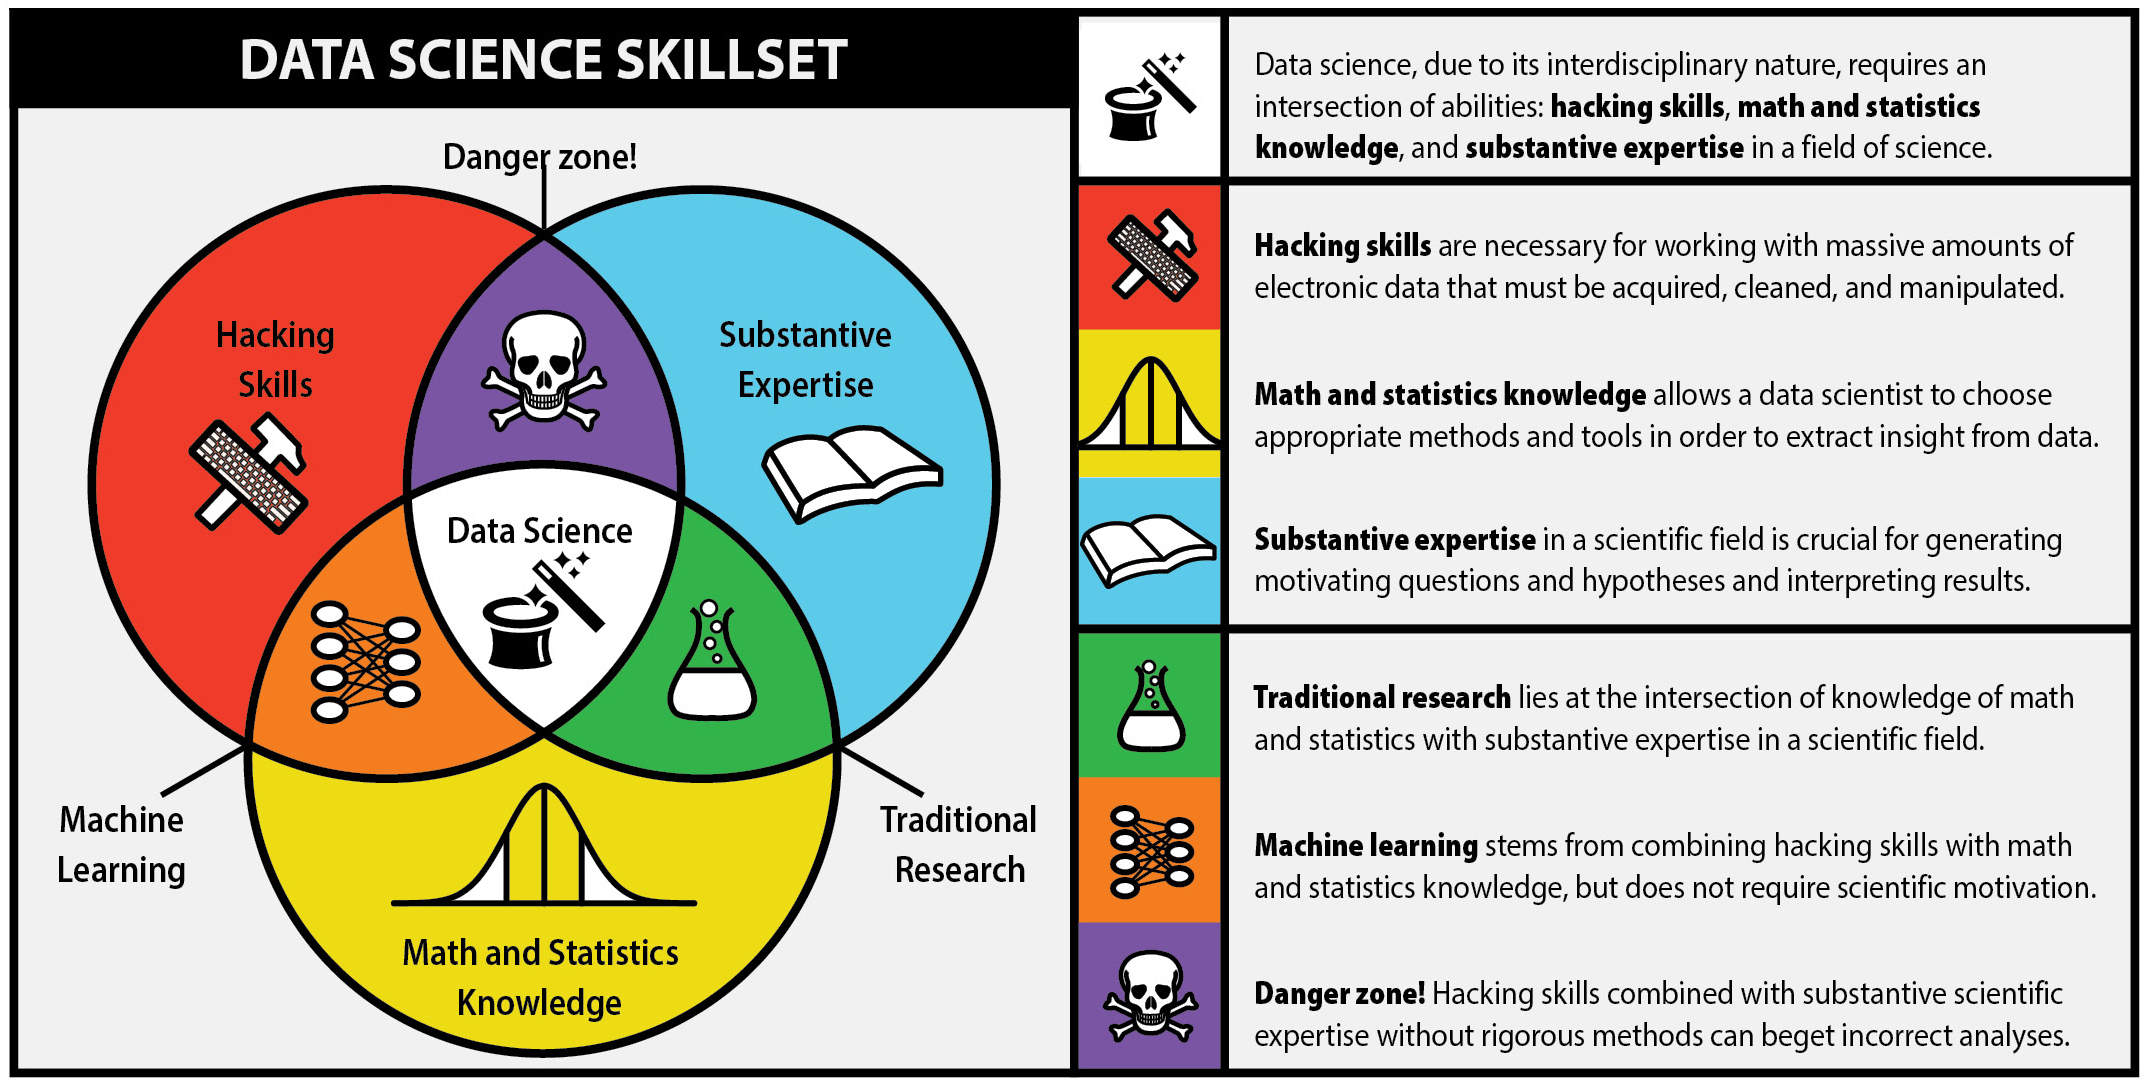
\includegraphics[width = .7\linewidth]{data-science-drew-conway.jpg}
\caption{Fuente: https://berkeleysciencereview.com/2013/07/how-to-become-a-data-scientist-before-you-graduate/ Original de Drew Conway.}
\end{figure}
}

\frame{
\frametitle{Finalmente}
\begin{figure}

\includegraphics[width = .3\linewidth]{reality-behind-data-science-70936148.png}
\end{figure}
}

\renewcommand{\section}[2]{}%
\appendix
\begin{frame}[allowframebreaks]
\frametitle{References}
% \bibliographystyle{apacite}
% \bibliography{bibliography.bib}
\printbibliography
\end{frame}


% ------------------------------------------------------------------------------
% ------------------------------------------------------------------------------
% ------------------------------------------------------------------------------
% ------------------------------------------------------------------------------
% ------------------------------------------------------------------------------

% ------------------------------------------------------------------------------



% ------------------------------------------------------------------------------
\begin{frame}[label=other-models]
\frametitle{Predicting gene functions}
There various approaches for this, some to highlight
\begin{itemize}%[<+->]
\item Text analysis like in \cite{Pesaranghader2016}
\item Protein-protein interaction networks like in \cite{Oliver2000,Piovesan2015}.
\item Phylogenetic based like SIFTER \cite{Engelhardt2005,Engelhardt2011}.
\begin{itemize}
\item Parameters to estimate: $2^{2P}$, where $P$ is the number of functions.
\end{itemize}
\end{itemize}

\vfill \hfill (a nice literature review in \cite{Jiang2016,Yu2018})
\hyperlink{aphylographicalview}{\beamerreturnbutton{go back}}

\end{frame}


% ------------------------------------------------------------------------------
\begin{frame}[label=aphyloalgorithmicview]
\frametitle{An evolutionary model of gene functions (algorithmic view)}

\scalebox{.7}{

\begin{algorithm}[H]
\SetAlgoLined
\KwData{A phylogenetic tree, $\{\pi, \mu, \psi\}$(Model probabilities)}
\KwResult{An annotated tree}
%\pause
\For{$n \in PostOrder(N)$}{
  $\mbox{\bf\color{usccardinal}Nodes gain/loss function depending on their parent}$\;%\pause
  \Switch{class of $n$}{
    \uCase{root node}{
      Gain function with probability $\pi$\;
    }%\pause
    \uCase{interior node} {%\pause
      \lIf{Parent has the function}{Keep it with prob. $(1-\mu_1)$}%\pause
      \lElse{Gain it with prob. $\mu_0$}%\pause
    }
  }%\pause
  $\mbox{\bf\color{usccardinal}Finally, we allow for mislabeling}$\;%\pause
  \uIf{$n$ is leaf}{%\pause
    \lIf{has the function}{Mislabel with prob. $\psi_1$}%\pause
    \lElse{Mislabel with prob. $\psi_0$}%\pause
  }
}
\end{algorithm}
}

\vfill\hfill \hyperlink{aphylographicalview}{\beamergotobutton{go back}}


\end{frame}




% ------------------------------------------------------------------------------


\end{document}

